\documentclass[tikz,border=10pt]{standalone}
\usepackage{amsmath}
\begin{document}
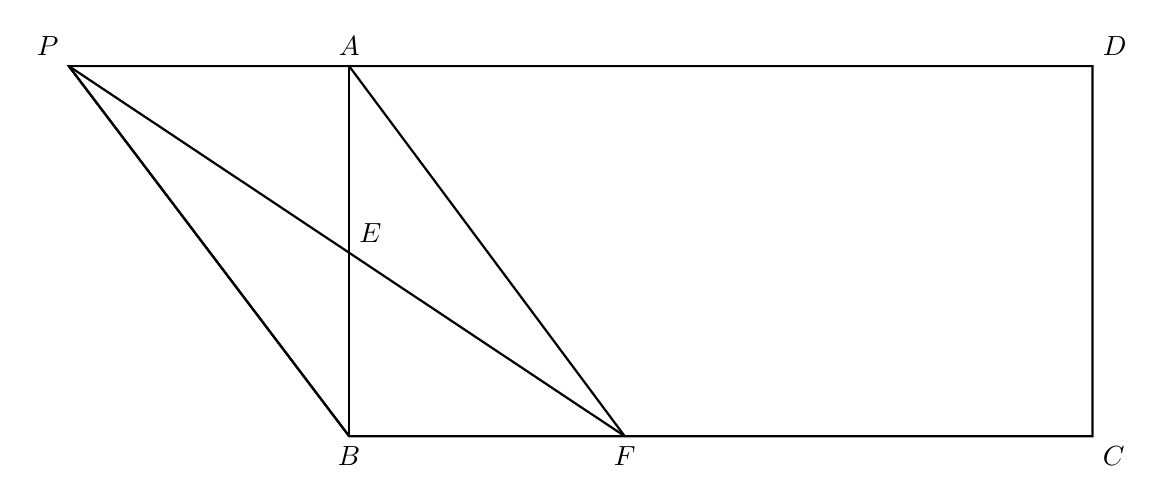
\begin{tikzpicture}[thick]
  \coordinate (P) at (-3.56,4.7);
  \coordinate (A) at (0,4.7);
  \coordinate (D) at (9.44,4.7);
  \coordinate (B) at (0,0);
  \coordinate (F) at (3.5,0);
  \coordinate (C) at (9.44,0);
  \coordinate (E) at (0,2.33);

  \draw (P) -- (A) -- (D) -- (C) -- (B) -- cycle;
  \draw (B) -- (A);
  \draw (P) -- (B);
  \draw (P) -- (F);
  \draw (A) -- (F);

  \node[above left] at (P) {$P$};
  \node[above] at (A) {$A$};
  \node[above right] at (D) {$D$};
  \node[below] at (B) {$B$};
  \node[below] at (F) {$F$};
  \node[below right] at (C) {$C$};
  \node[above right] at (E) {$E$};
\end{tikzpicture}
\end{document}
